%%%%%%%%%%%%%%%%%%%%%%%%%%%%%%
%%%%%%%%%%%%%%%%%%%%%%%%%%%%%%
\section{Neutrinos from the Sun and Earth --  theory}

There are several indirect methods for detection of neutralinos.
One of the most promising \cite{neutrinos} is to make use of the
fact that scattering of halo neutralinos by the Sun and the planets,
in particular the Earth, during the several
billion years that the Solar system has existed, will have trapped
these neutralinos within these astrophysical bodies. Being trapped
within the Solar or terrestrial material, they will sink towards
the center, where a considerable enrichment and corresponding
increase of annihilation rate will occur.


Searches for neutralino annihilation into neutrinos
will be subject to  extensive experimental investigations in view
of the new neutrino telescopes (AMANDA, IceCube, Baikal, NESTOR, ANTARES)
planned or under construction \cite{halzen}. A high-energy
neutrino signal in the direction of the centre of the Sun or Earth
is an excellent experimental signature which may stand up against
the background of neutrinos generated by cosmic-ray interactions in the
Earth's atmosphere.

There are several different approximations one could do, or processes to
include when calculating the capture rates in the Earth/Sun and many of these
are coded into \ds. The default in \ds\ is always to use the best calculations
available, but more approximate (older) routines are also available,
as well as more speculative signals, like the Damour-Krauss signal
(not included by default). If you want to use something else than the
defaults, or want to call more internal rotuines (more internal than
\code{dsntrates} or \code{dsntdiffrates}), you should read the
following sections carefully.


%%%%%%%%%%%%%%%%%%%%
\subsection{Neutrino yield from annihilations}

The differential neutrino flux from neutralino annihilation is
\beq
\frac{dN_\nu}{dE_\nu} =
\frac{\Gamma_A}{4\pi D^2} \sum_{f}
B^{f}_{\chi}\frac{dN^f_\nu}{dE_\nu}
\eeq
where $\Gamma_A$ is the annihilation rate,
$D$ is the distance of the detector from the source (the
central region of the Earth or the Sun), $f$ is the neutralino pair
annihilation final states,
and $B^{f}_{\chi}$ are the branching ratios into the final state $f$.
  $dN^f_\nu/dE_{\nu}$ are the energy
distributions of  neutrinos generated by the final state $f$ and are
obtained from the {\sc Pythia} simulations described in section
\ref{sec:mcsim}.

In comparison with calculations using the results of \cite{RS}
(e.g.\ ~\cite{neuprod}), this
Monte Carlo treatment of the neutrino propagation through the Sun
does not need the simplifying assumptions previously made, namely neutral
currents are no more assumed to be much weaker than charged currents
and energy loss is no more considered continuous.

The neutrino-induced muon flux may be detected in a neutrino telescope
by measuring the muons that come from the direction of the centre
of the Sun or Earth. For a shallow detector, this usually has to
be done in the case of the Sun by looking (as always the case for
the Earth) at upward-going muons, since there is a huge background
of downward-going muons created by cosmic-ray interactions in the
atmosphere. There is always in addition a more isotropic
background coming from muon neutrinos created on the other side of
the Earth in such cosmic-ray events (and also from cosmic-ray
interactions in the outer regions of the Sun).
The flux of muons at the detector is  given by

\beq
\frac{d N_\mu}{d E_\mu}
= N_A \int^\infty_{E_\mu^{\rm th}} d E_\nu
\int_0^\infty d\lambda \int_{E_\mu}^{E_\nu}
d {E'_\mu }\,\,
P(E_\mu,E'_\mu; \lambda)\,\,
\frac{d \sigma_\nu (E_\nu,E'_\mu)}{d E'_\mu} \,\,
\frac{d N_\nu}{d E_\nu}\, ,
\label{eq:muflux}
\eeq
where $\lambda$ is the muon range in the medium (ice or water
for the large detectors in the ocean or at the South Pole,
or rock which surrounds the smaller underground detectors),
$d \sigma_\nu (E_\nu,E'_\mu) / d E'_\mu$ is
the weak interaction cross section for production of a muon of
energy $E'_\mu$ from a parent neutrino of energy $E_\nu$, and
$P(E_\mu,E'_\mu; \lambda)$ is the
probability for a muon of initial energy $E'_\mu$
to have a final energy $E_\mu$ after passing
  a path--length $\lambda$ inside the detector medium.
$E_\mu^{\rm th}$ is the detector threshold energy, which for
``small''
neutrino telescopes like Baksan, MACRO and Super-Kamiokande is
around 1 GeV.
Large area neutrino telescopes in the ocean  or in Antarctic ice
typically
have thresholds of the order of tens of GeV, which makes them
sensitive mainly to heavy neutralinos (above 100 GeV)
\cite{begnu2}.

The integrand in Eq.~(\ref{eq:muflux}) is weighted towards high
neutrino energies, both because the cross section $\sigma_\nu$
rises approximately linearly with energy and because the average
muon energy, and therefore the range $\lambda$, also grow
approximately linearly with $E_\nu$. Therefore, final states
which give a hard neutrino spectrum (such as heavy quarks, $\tau$
leptons and $W$ or $Z$ bosons) are usually more important
than the soft spectrum arising from light quarks and gluons.

%%%%%%%%%%%%%%%%%%%%
\subsection{Evolution of the number density in the Earth/Sun}

Neutralinos are steadily being trapped in the Sun or Earth by
scattering, whereas annihilations take them away.
Let $N(t)$ be the total number of neutralinos trapped, at time $t$, in the core
of, for example,  the Earth.
The annihilation rate of neutralino pairs can be written as
\begin{equation}
\Gamma_a (t) = \frac{1}{2} \ C_a \, N^2 (t) \, . \label{eqx.1}
\end{equation}

The evolution of $N(t)$ is the result of the competition between capture and
annihilation:
\begin{equation}
\frac{dN}{dt} = C_c (t) - C_a \, N^2 \label{eqx.2}
\end{equation}
The constant $C_c$ is the capture rate, and
$C_a$ entering equations (\ref{eqx.1}) and (\ref{eqx.2}) is linked to
the annihilation cross-section $\sigma_a$, and to some effective volumes $V_j$,
$j=1,2$, taking into account the quasi-thermal distribution of neutralinos in
the Earth core:
\begin{equation}
C_a = \langle \sigma_a \, v \rangle \, \frac{V_2 }{ V_1^2} \, , \label{eq6.3}
\end{equation}
\begin{equation}
V_j \simeq 2.3 \times 10^{25} \, \left(\frac{j \, m_X}{ 10 \, {\rm 
GeV}}\right)^{-3/2} \, {\rm
cm}^3 \, . \label{eq6.4}
\end{equation}

This has the solution for the annihilation rate implemented in \ds\
\beq
\Gamma_A={C_c\over 2} \tanh^2\left({t\over \tau}\right),\label{eq:tanh}
\eeq
where the equilibration time scale $\tau=1/\sqrt{C_cC_a}$.  In most
cases for the Sun, and in the cases of observable fluxes for the
Earth, $\tau$ is much smaller than a few billion years, and therefore
equilibrium is often a good approximation ($\dot N(t)=0$).
This means
that it is the capture rate which is the important quantity that
determines the neutrino flux. However, in the program we keep the exact
formula (\ref{eq:tanh}), with some
modifications discussed in Sec.~\ref{sec:dk}).

%%%%%%%%%%%%%%%%%%%%
\subsection{Approximate capture rate expressions}

The capture rate induced by scalar (spin-independent) interactions
between the neutralinos and the nuclei in the interior of the Earth or
Sun is the most difficult one to compute, since it depends sensitively
on the Higgs mass, form factors, and other poorly known quantities.
However, this spin-independent capture rate calculation is the same as
for direct detection treated in Section~\ref{subs:direct}.  Therefore,
there is a strong correlation between the neutrino flux expected from
the Earth (which is mainly composed of spin-less nuclei) and the
signal predicted in direct detection experiments \cite{begnu2,kamsad}.
It seems that even the large (kilometer-scale) neutrino telescopes
planned, when searching for neutralino annihilation in the Earth, will
not be competitive with the next generation of direct detection
experiments when it comes to detecting neutralino dark matter.
However, the situation concerning the Sun is more favourable.  Due to
the low counting rates for the spin-dependent interactions in
terrestrial detectors, high-energy neutrinos from the Sun constitute a
competitive and complementary neutralino dark matter search.  Of
course, even if a neutralino is found through direct detection, it
will be extremely important to confirm its identity and investigate
its properties through indirect detection.  In particular, the mass
can be determined with reasonable accuracy by looking at the angular
distribution of the detected muons \cite{EG,BEK}.

For the Sun, dominated by hydrogen, the axial (spin-dependent)
cross section is important and relatively easy to compute.  A
reasonably good
approximation is given by \cite{jkg}
\beq
      {C^{\rm sd}_\odot\over (1.3\cdot 10^{23}\, {\rm s}^{-1})
\left(270\ {\rm km\,s^{-1}}/ \bar v\right)}=
\left({\rho_\chi\over 0.3\ {\rm GeV}\,{\rm cm}^{-3}}\right)
      \left({100\,{\rm GeV}\over m_\chi}\right)
\left({\sigma_{p\chi}^{\rm sd}\over 10^{-40}\ {\rm
      cm}^2}\right)
\eeq
where $\sigma_{p\chi}^{\rm sd}$ is the cross section for
neutralino-proton elastic scattering via the axial-vector interaction,
$\bar v$ is the dark-matter velocity dispersion, and $\rho_\chi$ is
the local dark matter mass.  The capture rate in the Earth is
dominated by scalar interactions, where there may be kinematic and
other enhancements, in particular if the mass of the neutralino almost
matches one of the heavy elements in the Earth.  For this case, a more
detailed analysis is called for, which is available in \cite{Gould87}
with convenient approximations in \cite{jkg}.
   In fact, also for the
Sun the spin-independent contribution can be important, in particular
iron may contribute non-negligibly.
For the Sun, the
  approximation in \cite{jkg} is also available,
\beqa
      {C^{\rm si}_\odot\over (4.8\cdot 10^{22}\, {\rm s}^{-1})
\left(270\ {\rm km\,s^{-1}}/ \bar v\right)}=
\left({\rho_\chi\over 0.3\ {\rm GeV}\,{\rm cm}^{-3}}\right)
      \left({100\,{\rm GeV}\over m_\chi}\right)\times & &\nonumber\\
\sum_A\left({\sigma_{A}^{\rm si}\over 10^{-40}\ {\rm
      cm}^2}\right)F_A(m_\chi)f_A\phi_AS\left(m_\chi/m_{A}\right)/m_{A},
\eeqa
where $f_A$ is the mass fraction of element $A$ and $\phi_A$ is the
typical gravitational potential (relative to the surface) for that
element. I.e.\ an element that is concentrated in the core will have a
higher $\phi_A$ than an element at the surface. $A$ is the atomic
number of the element and $M_{A}$ is its mass. The factor $S$ is a
kinematical suppression factor \cite{jkg,kamion91}. In the next
subsection we will go through the compositions of the Earth/Sun that
we use.

The approximate capture rate expressions above are coded into the routines
\code{dsntcapsun} and \code{dsntcapearth}. More accurate expressions
will follow in the coming subsections.


%%%%%%%%%%%%%%%%%%%%%%%%%%%%%%
\subsection{Earth and Sun composition}

When the capture rates are calculated, we need to know the composition
and density of the Earth/Sun as a function of depth.  

In \cite{jkg} they used average mass fractions and potentials for the
location of the various elements in the Sun. We have updated these to
the BP2000 \cite{bp2000} values instead, as given in Table~\ref{tab:suncomp}

\begin{table}
  \centering
  \begin{tabular}{lccc}
   & & \multicolumn{2}{c}{Average parameters} \\ \cline{3-4}
   Element & Mass number ($A$) & $f_i$ & $\phi_i$ \\ \hline
   Hydrogen, H       &  1 & 0.670    & 3.15 \\
   Helium-4, $^4$He  &  4 & 0.311    & 3.40 \\
   Carbon, C         & 12 & 0.00237  & 2.85 \\
   Nitrogen, N       & 14 & 0.00188  & 3.83 \\
   Oxygen, O         & 16 & 0.00878  & 3.25 \\
   Neon, Ne          & 20 & 0.00193  & 3.22 \\
   Magnesium, Mg     & 24 & 0.000733 & 3.22 \\
   Silicon, Si       & 28 & 0.000798 & 3.22 \\
   Sulphur, S        & 32 & 0.000550 & 3.22 \\
   Iron, Fe          & 56 & 0.00142  & 3.22 \\ \hline
\end{tabular}
\caption{The composition of the Sun with average parameters to be used
  in the approximative relations given in \cite{jkg}. These values are
  updated with the solar model of \cite{bp2000} and differs slightly
  from the values used in \cite{jkg}.}
  \label{tab:suncomp}
\end{table}

\begin{table}
  \centering 
  \begin{tabular}{lcccccc}
& Mass & \multicolumn{2}{c}{Mass fraction} & & \multicolumn{2}{c}{Average parameters}
\\ \cline{3-4} \cline{6-7}
 Element & number ($A$) & Core & Mantle & & $f_i$ & $\phi_i$ \\ \hline
  Oxygen, O     & 16 & 0.0   & 0.440   & & 0.298   & 1.20  \\
  Silicon, Si   & 28 & 0.06  & 0.210   & & 0.162   & 1.24  \\
  Magnesium, Mg & 24 & 0.0   & 0.228   & & 0.154   & 1.20  \\
  Iron, Fe      & 56 & 0.855 & 0.0626  & & 0.319   & 1.546 \\
  Calcium, Ca   & 40 & 0.0   & 0.0253  & & 0.0171  & 1.20  \\
  Phosphor, P   & 30 & 0.002 & 0.00009 & & 0.00071 & 1.56  \\
  Sodium, Na    & 23 & 0.0   & 0.0027  & & 0.00183 & 1.20  \\
  Sulphur, S    & 32 & 0.019 & 0.00025 & & 0.0063  & 1.59  \\
  Nickel, Ni    & 59 & 0.052 & 0.00196 & & 0.0181  & 1.57  \\
  Aluminum, Al  & 27 & 0.0   & 0.0235  & & 0.0159  & 1.20  \\
  Chromium, Cr  & 52 & 0.009 & 0.0026  & & 0.0047  & 1.44  \\ \hline
\end{tabular}
  \caption{The composition of the Earth's core and mantle. The core
    mass fractions are from \cite{earthcomp}[Table 4] and the mantle
    mass fractions are from \cite{earthcomp}[Table 2]. The average
    mass fractions and potentials in the last two columns are weighted
    averages assuming a core mass of $1.93\cdot10^{24}$ kg and a
    mantle mass of $4.04\cdot10^{24}$ kg with average potentials
    (relative to the surface) of 1.6 in the core and 1.2 in the mantle
    \cite{Gould87}.} \label{tab:earthcomp} 
\end{table}

For the Earth, we have also implemented more accurate
density profiles and more up-to date chemical distributions within the
Earth. We use the estimates for the Earth composition given in
\cite{earthcomp}[Table 2 for the mantle and Table 4 for the core]. In
Table~\ref{tab:earthcomp} we list these values together with the
average parameters $f_i$ and $\phi_i$ that should be used in the
expressions for the approximate capture rates in the previous
section. Note that using these average parameters instead of
integrating over the full radius is equivalent to putting all the
elements of the give type at the gravitational potential $\phi_i$.

\begin{figure}
\centerline{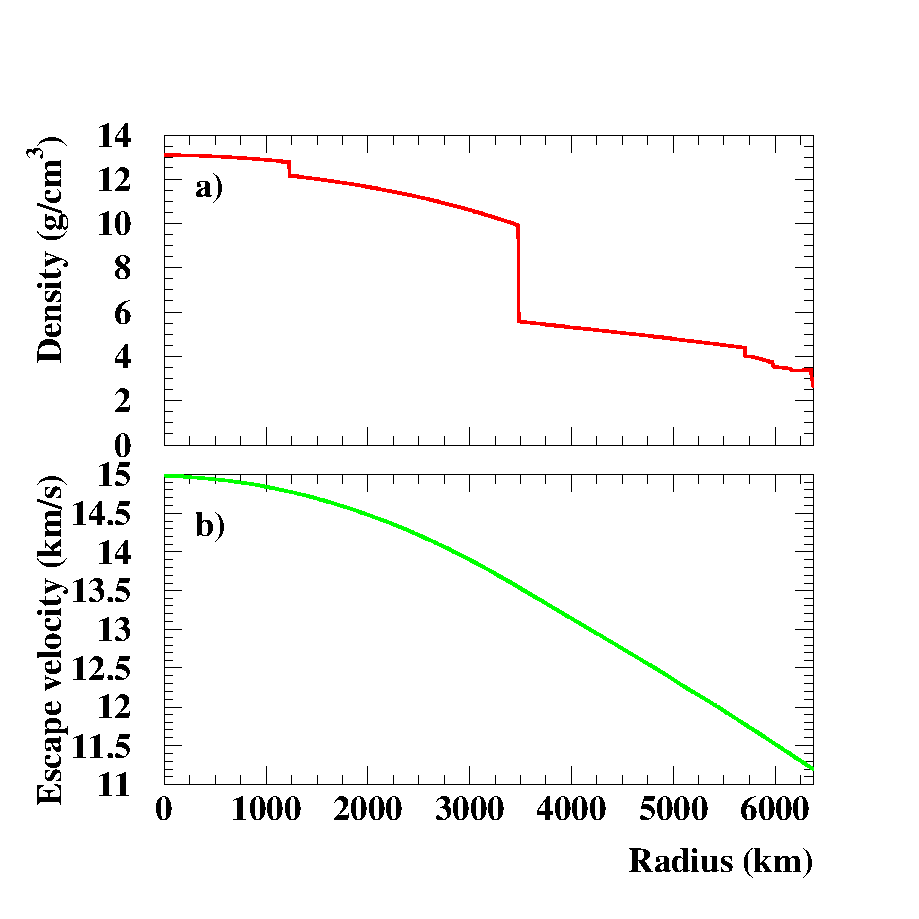
\epsfig{file=fig/eadensvesc.eps,width=0.6\textwidth}}
\caption{In a) the density profile and in b) the escape velocity in the Earth is shown.}
\label{fig:eadensvesc}
\end{figure}

We also need the density profile of the Earth, and for this we use the
values in \cite{EncBrit}. Using this density profile, we can calculate
the gravitational potential, $\phi(r)$ inside the Earth and from this
one the escape velocity $v$ inside the Earth,
\begin{equation}
   \label{eq:vesc}
   v = 11.2 \sqrt{\frac{\phi(r)}{\phi(R_\oplus)}} \mbox{~km/s.}
\end{equation}
In Fig.~\ref{fig:eadensvesc} we show the density profile and escape
velocity inside the Earth. 

%%%%%%%%%%%%%%%%%%%%%%%%%%%%%%%%%%%%%%%%
\subsection{More accurate capture rate expressions}

Another complicating factor when calculating the capture rates is the
integration over the velocity 
distribution. In \cite{Gould87}, parts of the integrations are
performed analytically for a Gaussian veolocity distributions. These
expressions are also coded in \ds for the Earth and give a more
accurate calculation of the capture rate in the Earth than the
approximations given above. The routine \code{dsntcapearth2} performs
these calculations for the Earth.

%%%%%%%%%%%%%%%%%%%%%%%%%%%%%%
\subsection{Accurate capture rates in the Earth for general velocity distributions}


If one wants even more accurate and general expressions for the
capture rates in the Sun/Earth, we have also implemented the full
expressions in \cite{Gould87}, but without assuming that the velocity
distribution is a Gaussian (or Maxwell-Boltzmann). These routines are
now the default in \ds.

We will here outline how these expressions look
like for the Earth and how they can be used both for a Maxwell-Boltzmann
distribution and for a general velocity distribution. The expressions
will of course look analogously for the Sun. We start with
the general case and study the special case of a Maxwell-Boltzmann
distribution in the next section. 

We will divide the Earth into shells and calculate the capture from
element $i$ in each shell individually. At the end we will integrate
over all the shells and sum over all the elements in the Earth. The
capture rate from element $i$ per unit shell volume is given by
\cite{Gould87}[Eq.~(2.8)] 
\begin{equation}
\label{eq:dcdv}
    \frac{dC_i}{dV} = \int_0^{u_{max}} du \frac{f(u)}{u} w \Omega_{v,i}^-(w)
\end{equation}
where $f(u)$ is the velocity distribution (normalized such that
$\int_0^\infty\ f(u) = n_\chi$ where $n_\chi$ is the number density of
WIMPs. The expression $\Omega_{v,i}^-(w)$ is related to the
probability that we scatter to orbits below the escape velocity. $w$
is the velocity at the given shell and it is related to the velocity
at infinity $u$ and the escape velocity $v$ by 
\begin{equation}
\label{ }
   w = \sqrt{u^2 + v^2}.
\end{equation}
The upper limit of integration is a priori set to $u_{max} = \infty$,
but we will see below that due to kinematical reasons we can set it to
a lower value (Eq.~(\ref{eq:umax}) below). 
If we allow for a form factor suppression of the form \cite{Gould87}[Eq.~(A3)]
\begin{equation}
\label{ }
   |F(q^2)|^2 = \exp\left( - \frac{\Delta E}{E_0} \right)
\end{equation}
with \cite{Gould87}[Eq.~(A4)]
\begin{equation}
\label{ }
   E_0 = \frac{3 \hbar^2}{2m_\chi R^2}
\end{equation}
we can evaluate $w \Omega_{v,i}^-(w)$ and arrive at the expression
\cite{Gould87}[Eq.~(A6)] 
\begin{equation}
\label{eq:womega}
   w \Omega_{v,i}^- (w) = \sigma_i n_i \frac{\mu_+^2}{\mu}2 E_0 \left[
   e^{- \frac{m_\chi u^2}{2E_0}} - e^{-\frac{\mu}{\mu_+^2}m_\chi \frac{u^2+v^2}{2E_0}}
   \right] \Theta\left( \frac{\mu}{\mu_+^2} - \frac{u^2}{u^2+v^2} \right)
\end{equation}
where we have introduced
\begin{equation}
\label{ }
   \mu = \frac{m_\chi}{m_i} \quad ; \quad \mu_\pm = \frac{\mu \pm 1}{2}
\end{equation}
with $m_i$ the mass of element $i$. The Heaviside step function
$\Theta$ plays the role of only including WIMPs that can scatter to a
velocity lower then the escape velocity $v$. To simplify our
calculations we can drop this step function in Eq.~(\ref{eq:womega})
and instead set the upper limit of integration in Eq.~(\ref{eq:dcdv})
to 
\begin{equation}
\label{eq:umax}
  u_{max} = \sqrt{\frac{\mu}{\mu_-^2}} v
\end{equation}
We also need the scattering cross section on element $i$, which can be
written as 
\cite{jkg}[Eq.~(9-25)]
\begin{equation}
\label{eq:sigma_i}
   \sigma_i = \sigma_p A_i^2 \frac{(m_\chi m_i)^2}{(m_\chi+m_i)^2} 
   \frac{(m_\chi + m_p)^2}{(m_\chi m_p)^2}
\end{equation}
where $A_i$ is the atomic number of the element, $m_p$ is the proton
mass and $\sigma_p$ is the scattering cross section on protons. 

We now have what we need to calculate the capture rate. In
Eq.~(\ref{eq:dcdv}) we integrate over the velocity for our chosen
velocity distribution. We then integrate this equation over the radius
of the Earth and sum over all the different elements in the Earth, 
\begin{equation}
\label{ }
   C = \int_0^{R_\oplus} dr \sum_i \frac{dC_i}{dV} 4 \pi r^2
\end{equation}
Note that we have not assumed anything special about our velocity
distribution, it doesn't even have to be isotropic since the
distribution of elements evenly in the shells will make an anisotropic
distribution on average to behave as an isotropic one. 

The routines that calculate the capture rates with these general (and
accurate) expressions are \code{dsntcapearthnum} and
\code{dsntcapsunnum}. As these calculations are somewhat
time-consuming, we have also added a possibility to tabulate the
result and interpolate in these tables. To use (or create, if the
table files are missing) instead call \code{dsntcapearthtab} and
\code{dsntcapsuntab}. These last two routines are the default in
\ds. The velocity distribution used is determined by a switch when the
halo model is set (i.e.\ when \code{dshmset} is called).


%%%%%%%%%%
\subsection{Accurate capture rates for the Earth for a
  Maxwell-Boltzmann velocity distribution}

We will here give some more information on how the approximations
introduced in the beginning of this chapter are derived from the
general expressions in the preceeding section.

If the velocity distribution is of Maxwell-Boltzmann type we can
greatly simplify our expressions above as we can perform the
integration over velocity analytically. The integration over radius
can also be further simplified by using the average mass fractions
$f_i$ and potentials $\phi_i$ in Tables~\ref{tab:suncomp}--\ref{tab:earthcomp}. 

If the velocity distribution in the halo is Maxwell-Boltzmann, it looks like
\begin{equation}
\label{ }
   f_h(u) du = n_\chi \frac{4}{\sqrt{\pi}} \left(\frac{3}{2}\right)^{\frac{3}{2}}
   \frac{u^2}{\bar{v}^3}
   e^{-\frac{3}{2}\frac{u^2}{\bar{v}^2}} du
\end{equation}
where $\bar{v}$ is the three-dimensional velocity dispersion and
$n_\chi$ is the number density of WIMPs in the halo. However, the
solar system moves through the halo with a velocity $v_*$ and the
distribution on observer with this velocity through the halo will see
is 
\begin{equation}
\label{eq:fstaru}
  f_*(u) = f_h(u) e^{-\frac{3}{2}\frac{v_*^2}{\bar{v}^2}} 
  \frac{\sinh\left(\frac{3 u v_*}{\bar{v}^2}\right)}{\frac{3 u v_*}{\bar{v}^2}} =
  n_\chi \sqrt{\frac{3}{2\pi}} \frac{u}{\bar{v} v_*} \left[
  e^{-\frac{3}{2} \frac{( u-v_*)^2}{\bar{v}^2}} -
  e^{-\frac{3}{2} \frac{( u+v_*)^2}{\bar{v}^2}} \right]
\end{equation}
Now one would naively believe that this is not the distribution that
an observer at the Earth will see. First of all, the Earth is moving
with respect to the Sun and secondly, the WIMPs have gained speed by
the gravitational attraction of the Sun when they reach the
Earth. Both of these arguments are true and the distribution of WIMPs
in the halo will not look like Eq.~(\ref{eq:fstaru}) to an observer on
the Earth. However, Gould \cite{Gould91} showed that WIMPs from the
halo can diffuse into the solar system due to gravitational
interactions with the planets and this distribution of WIMPs will
roughly look like as if the Earth was in free space moving through the
halo with the velocity of the solar system,
i.e.\ Eq.~(\ref{eq:fstaru}). We will later scrutinize this statement,
as it turns out that it does not quite hold, but 
as a first guess it is a reasonable approximation. For the Sun,
though, the velocity distribution give above is the correct one for a
Maxwell-Boltzmann distribution.

With the distribution Eq.~(\ref{eq:fstaru}) we can analytically
perform the integration over velocity in Eq.~(\ref{eq:dcdv}). After
some algebra we arrive at \cite{Gould87}[Eq.~(A10)] 
\begin{eqnarray}
\frac{dC_i}{dV} & = & \left( \frac{8}{3\pi} \right)^{\frac{1}{2}} 
\frac{\sigma_i n_i n_\chi \bar{v}}{2b\eta} \nonumber \\
 & & \Bigg[ \frac{e^{-a\hat{\eta}^2}}{\sqrt{1+a}} \left[ 2 \widetilde{\rm erf}(\hat{\eta}) - \widetilde{\rm erf} (\hat{A}_+) + \widetilde{\rm erf} (\hat{A}_-) \right]
   \nonumber \\ 
& &  - \frac{e^{-b\check{\eta}^2}}{\sqrt{1+b}}
   e^{-(a-b)A^2} \left[ 2 \widetilde{\rm erf}(\check{\eta}) - \widetilde{\rm erf} (\check{A}_+) + \widetilde{\rm erf} (\check{A}_-)
   \right] \Bigg]
   \label{eq:dcdvmb}
\end{eqnarray}
where $\widetilde{\rm erf}$ is the modified error function,
\begin{equation}
\label{eq:moderf}
   \widetilde{\rm erf} (x) = \frac{\sqrt{\pi}}{2} {\rm erf} (x)
   \qquad ; \qquad {\rm erf}(x) = \frac{2}{\sqrt{\pi}} \int_0^x e^{-y^2} dy.
\end{equation}
Following Gould \cite{Gould87}, we have in Eq.~(\ref{eq:dcdvmb})
introduced the following shorthand notation: 
\begin{equation}
\begin{array}{ccccc}
\eta = \sqrt{\frac{3}{2}} \frac{v_*^2}{\bar{v}^2} & ; &
a = \frac{m_chi \bar{v}^2}{3E_0} & ; & b=\frac{\mu}{\mu_+^2} a \\
\hat{\eta} = \frac{\eta}{\sqrt{1+a}} & ; & \check{\eta} = \frac{\eta}{\sqrt{1+b}} \\
A^2 = \frac{3}{2} \frac{v^2}{\bar{v}^2} \frac{\mu}{\mu_-^2} & ; &
\hat{A} = A \sqrt{1+a} & ; & \check{A} = A \sqrt{1+b} \\
\hat{A}_\pm = \hat{A} \pm \hat{\eta} & ; & \check{A}_\pm = \check{A} \pm \check{\eta}
\end{array}
\end{equation}
If we wish, we can now integrate Eq.~(\ref{eq:dcdvmb}) over radius
just like in the previous section, but we can without loosing too much
accuracy, replace this integration with a sum over the elements in the
Earth with their respective typical location. I.e.\ we can write 
\begin{equation}
\label{ctotmb}
  C = \sum_i \frac{dC_i}{dV}\frac{1}{n_i} \frac{f_i M_\oplus}{m_i}  
\end{equation}
where we instead of the number density $n_i$ use the total number of
atoms of the given type $f_i M_\oplus/m_i$. Note that for each element
in the sum we should evaluate this expression at the given typical
gravitational potential $\phi_i$ of the element, i.e.\ with the escape
velocity given by Eq.~(\ref{eq:vesc}). The mass fractions $f_i$ and
typical potentials $\phi_i$ are listed in Table
\ref{tab:earthcomp} (and analogously in Table~\ref{tab:suncomp} for
the Sun). This approximation introduces an error of no more
than about 1--2\% for a Maxwell-Boltzmann distribution\footnote{Note
  that it is not advisable to use this approximation for general
  velocity distributions. If one e.g.\ has a lower limit on possible
  velocities, $u_{min}$, for heavy WIMPs capture will then only be
  possible very close to the central core. Replacing the actual
  distribution of potentials $\phi(r)$ with the typical value $\phi_i$
  may then introduce larger errors. We will encounter these kind of
  distributions shortly.} 

The capture rate evaluated with the expressions shown here are encoded
into the routine \code{dsntcapearth2}. Note that we have not coded the
corresponding approximate expressions for the Sun. Instead, as given
in the preceeding section, we now have more accurate expressions for
both the Sun and the Earth.

%%%%%%%%%%%%%%%%%%%%%%%%%%%%%%
\subsection{A possible new population of neutralinos}\label{sec:dk}

Recently, it has been shown that the scattering process in the Sun can
populate orbits which subsequently result in a bound Solar System
population of WIMPs~\cite{dk1,dk2} and which can be comparable in
spectral density, in the region of the Earth, to the Galactic halo
WIMP population.  This new population consists of WIMPs that have
scattered in the outer layers of the Sun and due to perturbations by
the other planets (mainly Venus and Jupiter) evolve into bound orbits
which do not cross the Sun but do cross the Earth's orbit.  This
population of WIMPs should have a completely different velocity
distribution than halo WIMPs and will thus have quite different
capture probabilities in the Earth.  The predicted WIMP abundance, and
spectrum, relevant for direct detection have been calculated in
\cite{dk1,dk2}, where it was shown that although the total rates may
not change by a large amount, there could be a striking directional
effect, which could be of impoertance once detectors with directional
sensitivity are built.  Also for capture in the Earth, and the
predicted indirect neutrino signature, there are poissibly large
effects, incorporated as an optional choice in \ds, coming from this
new population \cite{dkpop}.  (Other studies of solar system
populations of WIMPs can be found in \cite{otherpop,Gould91}.  See
also the comments in \cite{gouldnew} about the uncertainties involved
in estimating these effects.)

The enhancement caused by the new population is only important for
neutralino mass less than 150 - 170 GeV (the exact number depending on
details about the angular momentum distribution \cite{dkpop}).

Following the notation of~\cite{dk1,dk2} one can write the
contribution from the new population of neutralinos to the usual halo
neutralino density as
\begin{equation}
   \delta_E \equiv \frac{n (a_1)}{n_X} \equiv \frac{\hbox{(secondary) neutralino
   density at the Earth}}{\hbox{halo neutralino density at infinity}} \, ,
   \label{eq5.11}
\end{equation}
where
\begin{equation}
   \delta_E = \frac{5.44 \times 10^{36}}{(v_o / 220 \, {\rm km\,s}^{-1})}
   \times
   g_{\rm tot} \, {\rm GeV} \, {\rm cm}^{-2} = \frac{0.212}{(v_o / 220 \,
   {\rm km\,s}^{-1})} \, g_{\rm tot}^{(-10)} \, . \label{eq5.15}
\end{equation}
Here, $g_{\rm tot}^{(-10)} \equiv 10^{10} \, g_{\rm tot} ({\rm
GeV})^3$, and $g_{\rm tot} = { \sum_A} \, (f_A / m_A) \, \sigma_A \,
\phi_A^s$, where $f_A$ is the mass fraction of element $A$ in the Sun,
and $\phi_A^s$ is the surface value of the capture function on the
element of mass number $A$ in the Sun \cite{dk2}.

The scattering rate of neutralinos in the outer layers of the Sun (which
causes the fast halo neutralinos to lose enough energy to enter bound orbits
close to the Earth's orbit) is proportional to $\sigma_A \phi_A^s$, which
can be calculated once the parameters of the SUSY neutralino in question are
fixed. (For the elemental abundances in the Sun, we use the compilation
in~\cite{jnb}.)

The values of $g_{\rm tot}^{(-10)}$
can in some cases approach unity. The spread is
very large, however, and some models give orders of magnitude smaller
values. As would be expected, the models with the highest values of
$g_{\rm tot}^{(-10)}$ are the same models which give high scattering
rates in direct detection experiments.
As mentioned, the integrated effect of the
new population in direct experiments is not very prominent
(see refs.~\cite{dk1,dk2}). On
the other hand,  they can imply a large effect
on indirect detection neutrino rates.

The total capture rate  is computed according
to the formulas in \cite{dkpop}, which take into account that the annihilation
rates from the earth will, in general depend on time in a different
way than the simple result in Eq.~(\ref{eq:tanh}).

Due to this nonlinear nature of the capture rate, there is no simple
scaling of the computed detection rates with the local halo density.
Therefore, it is advisable that the user rescales the local halo
density (see section \ref{sec:rescale}) before calculating the rates
in neutrino telescopes.

The new population can cause an increase of the detection rates
by as much as a factor of 100 when the neutralino mass is less
than around 150 GeV\@.


%%%%%%%%%%%%%%%%%%%%%%%%%%%%%%
\subsection{Effects of WIMP diffusion in the solar system}

As the Earth has a rather low escape velocity, the Earth will only be
able to capture WIMPs that have a rather low velocity with respect to
the Earth. However, WIMPs from the halo have gained speed in the
gravitaional potential from the Sun and will essentially be impossible
to capture by the Earth. Hence, the Earth will only capture WIMPs that
have diffused around in the solar system (by gravitational
interactions with the other planets). Gould showed \cite{gould-diff}
that effectively this diffusion will lead to the same phase space
distribution at the Earth as if the Earth was in free space
(i.e.\ neglecting the solar potential). However, numerical simulations
of asteroids showed that they are thrown into the Sun due to
perturbations of the orbits by other planets, see
e.g.\ \cite{farinella}. These analyses led to worried that maybe the
population of WIMPs diffusing around in the solar system is not as big
as thought \cite{gould-conserv}. In \cite{earth-diff}, Lundberg and
Edsj\"o investigated this issue with detailed numerical simulations of
WIMP orbits in the solar system, showing that the annihilation rate in
the Earth is typically reduced by up to two orders of magnitude. In
\ds, we include these results for the neutrino rates from the Earth by
using the velocity distribution at the Earth (as obtained in
\cite{earth-diff}). This velocity distribution is then used as input
for our numerical capture rate routines instead of the usual
approximation of using the halo velocity distribution directly. Using
these new velocity distributions for the Earth is the default in \ds.
